\chapter{Experimentální měření}

\section{Metodologie}

Pro účely testování jsme využili proces soutěže SMT-COMP\footnote{\url{https://smt-comp.github.io/}}, která od roku 2005 každoročně srovnává nejlepší současné SMT řešiče na velkém množství různorodých testů z knihovny SMT-LIB. Náš řešič porovnáváme v kategorii diferenční logiky s řešiči, které se účastnili soutěže v roce 2020. Konkrétně to jsou řešiče CVC4, MathSAT5, SMTInterpol, veriT, Yices a z3.

Náš experiment proběhl na 834 testovacích vstupech knihovny SMT-LIB určených pro diferenční logiku. Samotné výpočty probíhaly na počítačích clusteru StarExec\footnote{\url{https://www.starexec.org/}}, iniciativy vzniklé za účelem jednoduššího vytváření, vyhodnocování a sdílení testů pro různé druhy logických řešičů. Počítače, jež jsou součástí clusteru, obsahují 2.4~GHz procesor Intel\textregistered Xeon\textregistered E5-2609 a cca.~250 GB operační paměti.

Omezení stanovená pro testy jsme rovněž převzali z SMT-COMP. Každý test byl spuštěn s limitem 1200~s reálného času, respektive 4800~s procesorového času a s omezením na 60~GB paměti. Výpočet prohlásíme za úspěšně dokončený, pokud skončil v rámci daných limitů a vrátil korektní odpověď. Jakmile je některý z limitů porušen, popřípadě není-li vrácená odpověď korektní, označili jsme test za neúspěšný. 

\section{Výsledky}

\begin{table}[h]
	\centering
	\begin{tabular}{l@{\hspace{1cm}} D{.}{,}{3.0} D{.}{,}{6.1} D{.}{,}{3.0} D{.}{,}{3.0} D{.}{,}{3.0}}
		\toprule  
		& \mc{\textbf{Úspěšně}} & \mc{\textbf{Reálný}} & \mc{\textbf{Vyřešeno}} & \mc{\textbf{Vyřešeno}} & \mc{} \\
		\pulrad{\textbf{Řešič}} &\mc{\textbf{vyřešeno}} & \mc{\textbf{čas}} & \mc{\textbf{SAT}} & \mc{\textbf{UNSAT}} & \mc{\pulrad{\textbf{Timeout}}}\\
		\midrule
		Yices & 740 & 128683.6 & 484 & 256 & 94 \\
		z3 & 727 & 124296.1 & 485 & 242 & 82 \\
		CVC4 & 682 & 231953.6 & 425 & 257 & 152\\
		\textbf{OpenSMT} & 661 & 260896.8 & 412 & 249 & 173 \\
		veriT & 621 & 308952.9 & 372 & 249 & 213\\
		MathSAT & 585 & 337559.4 & 341 & 244 & 249\\
		SMTInterpol & 546 & 396759.1 & 313 & 233 & 288\\
		\bottomrule
	\end{tabular}
	%\caption{Srovnání SMT řešičů}
\end{table}

{
	\centering
		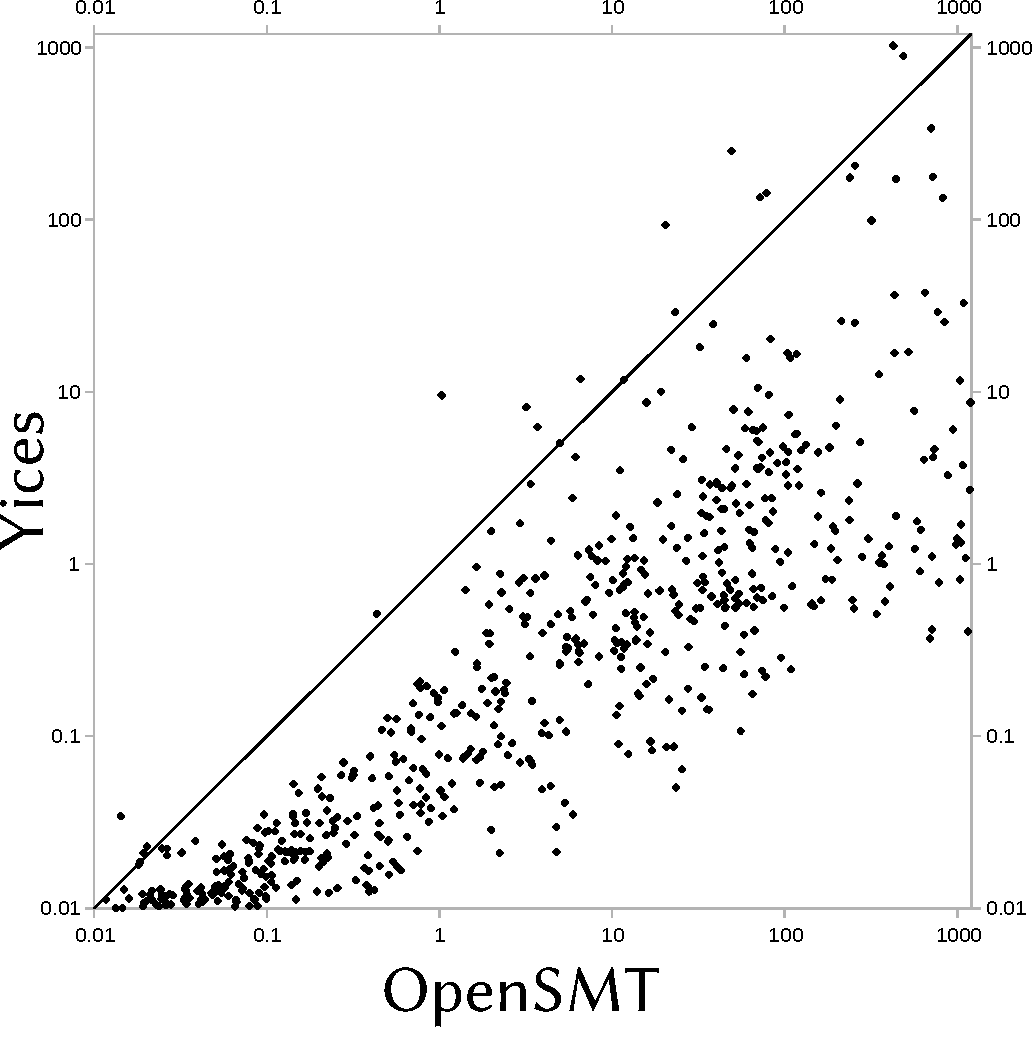
\includegraphics[width=0.49\linewidth]{comp_yices}
		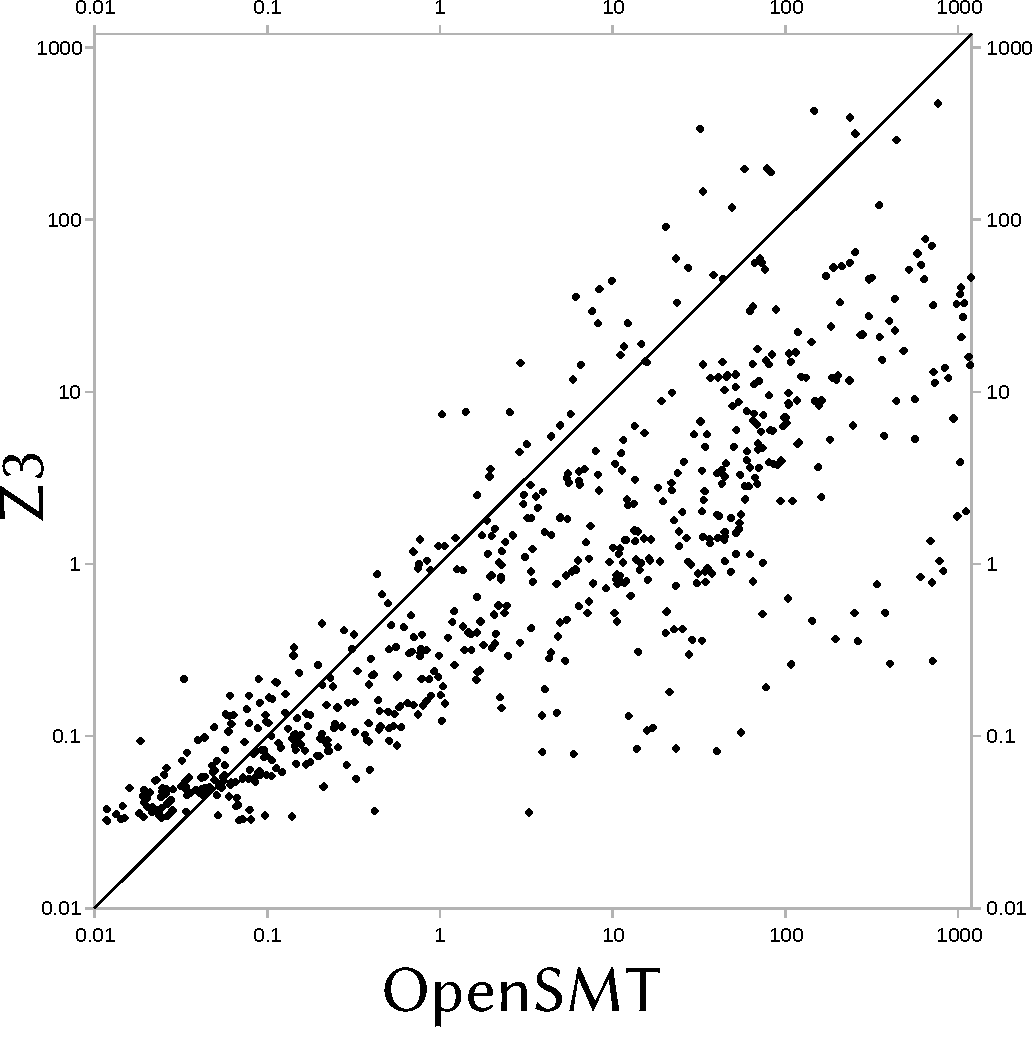
\includegraphics[width=0.49\linewidth]{comp_z3}\\
		\vspace{5px}
		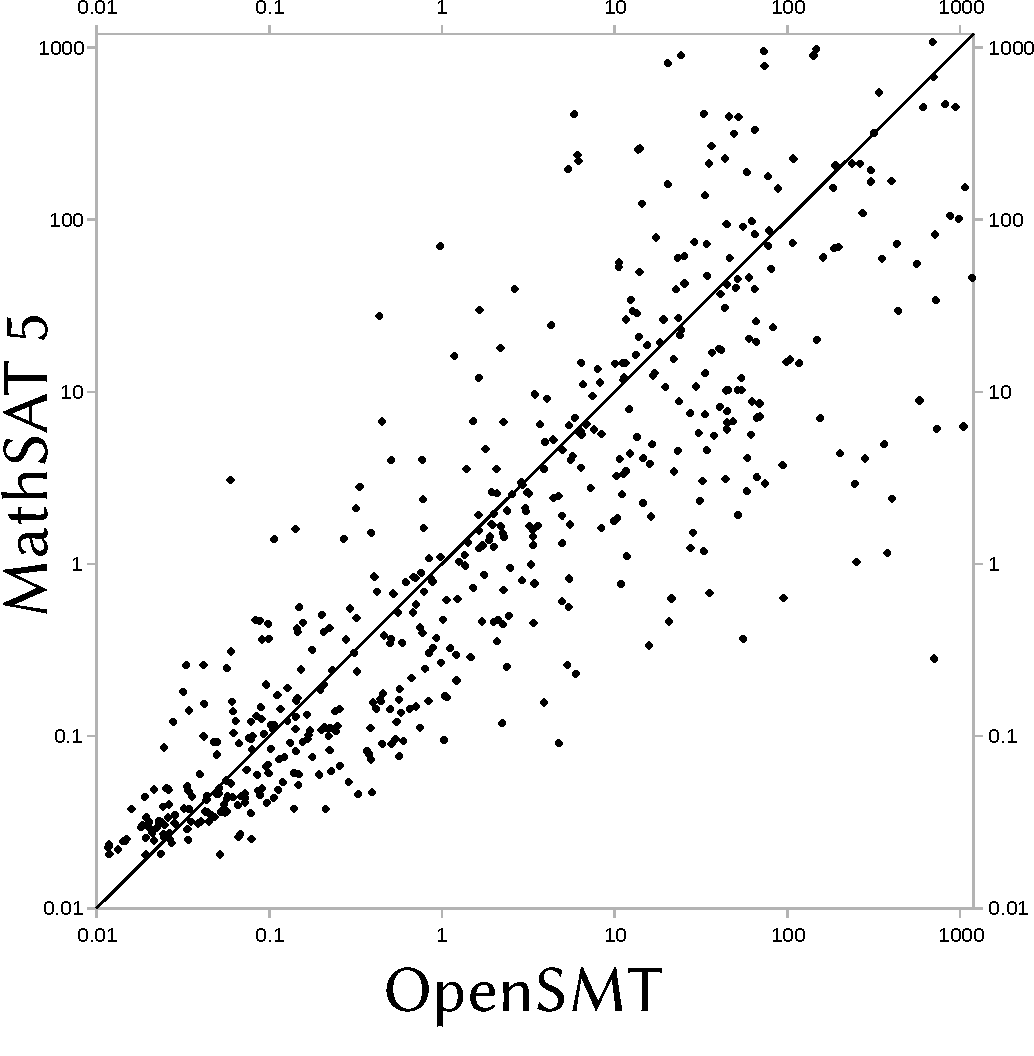
\includegraphics[width=0.49\linewidth]{comp_mathsat}
		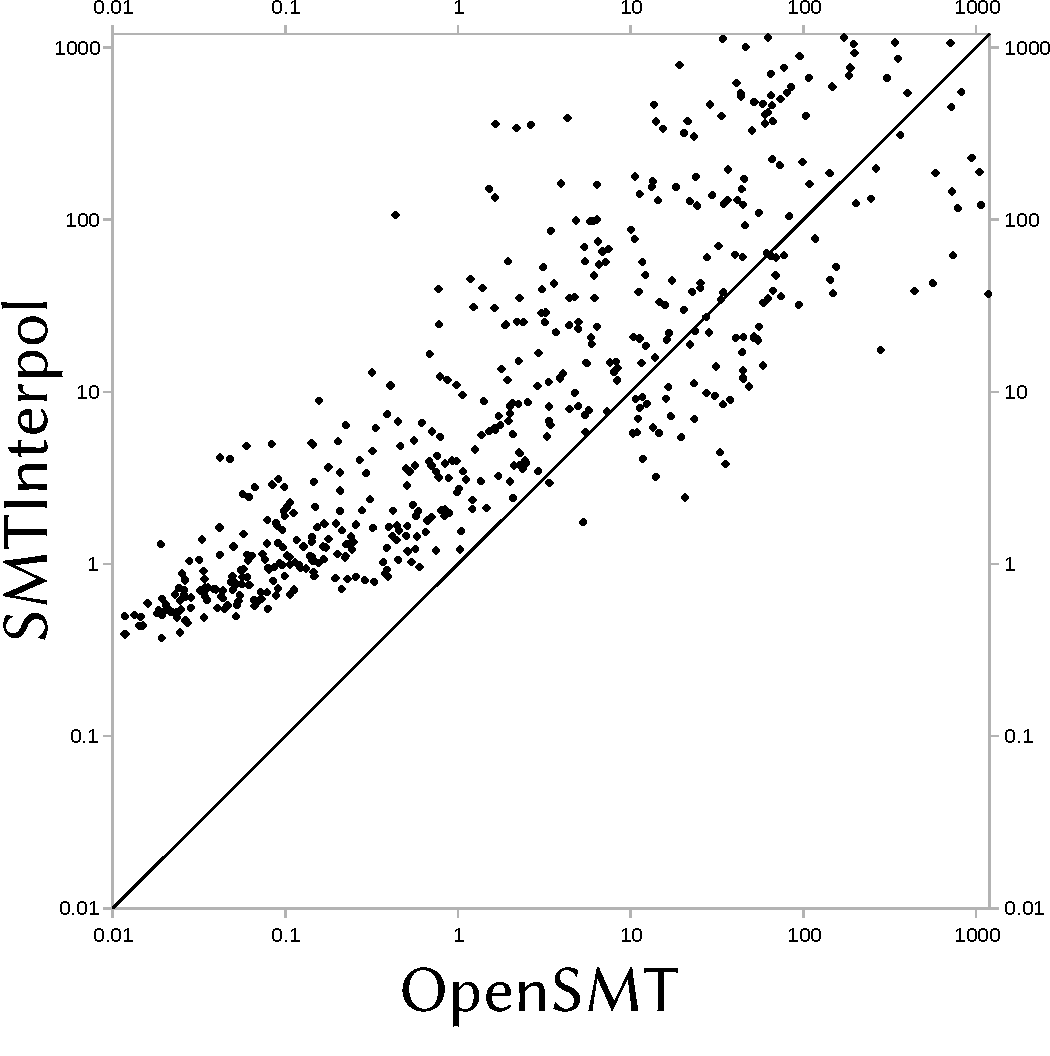
\includegraphics[width=0.49\linewidth]{comp_smti}\\
		\vspace{5px}
		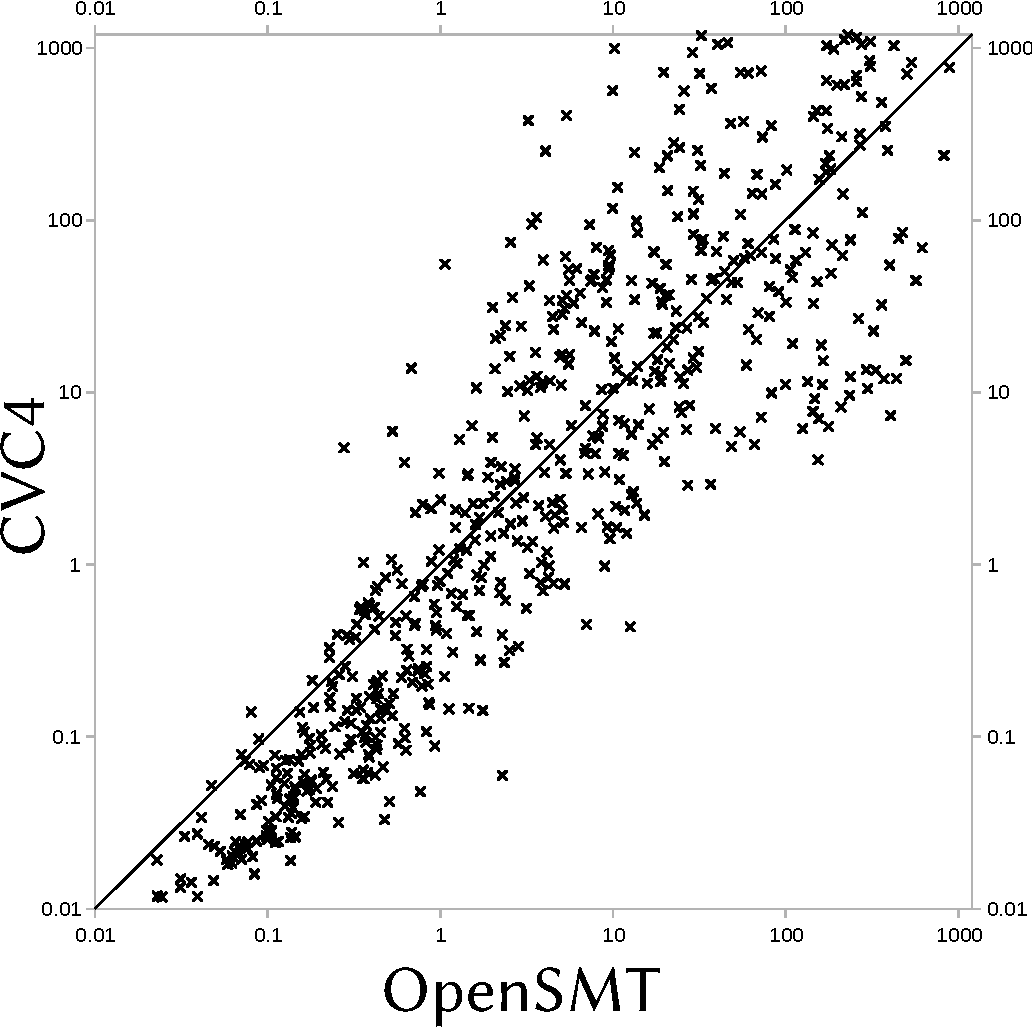
\includegraphics[width=0.49\linewidth]{comp_cvc}
		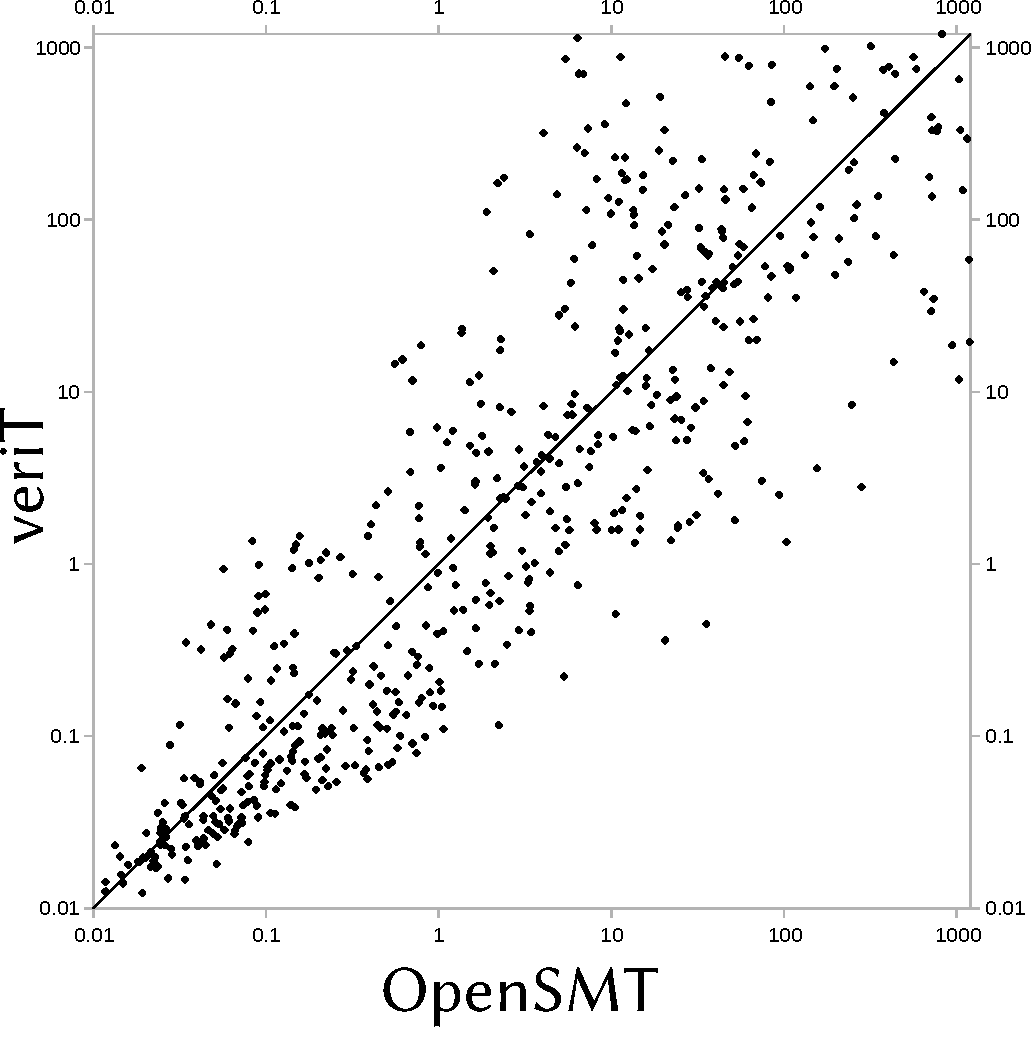
\includegraphics[width=0.49\linewidth]{comp_verit}\\
}
\section{Srovnání}
